\documentclass[../Main/Main.tex]{subfiles}

\begin{document}
En luz de las nuevas y populares tendencias en el mundo de la estadística computacional, a veces llamada \textit{Aprendizaje de Maquina o Machine Learning (ML)}, este trabajo, busca desarrollar y entender desde sus cimientos, un modelo aplicable a esta categoría. Este modelo, buscará hacer inferencia sobre una base de datos y \textit{aprender} sobre los patrones subyacentes que estos puedan contener. Se busca revisar todos los aspectos de su construcción: tanto consideraciones teóricas e históricas hasta diferentes paradigmas de aprendizaje; así como su implementación y validación en una computadora. Todo esto, para dar un contexto sobre la, también llamda, \textit{Inteligencia Artificial}, lo cual no es más que estadística computacional llevada al límite. \\

Este tipo de modelos, han resultado ser de enorme efectividad en  ámbitos que van, desde la medicina hasta las finanzas. Sin embargo, en ocaciones, los métodos de ML son tratadas como \textit{cajas negras}; se tienen datos que se alimentan a un modelo complejo y este arroja resultados. Aunque estos métodos son útiles, el tratamiento de los datos y el modelo en si, no se debe dejar de un lado, pues existen consideraciones técnicas y supuestos que se deben cumplir. Además, la interpretación, validación y análisis de los resultados, deben ser realizados por alguien que conozca, al menos de manera general, que está haciendo la computadora.\\

En particular, el modelo que se presenta a continuación, busca la predicción de variables binarias en un contexto de regresión bayesiana a través de un proyector aditivo con una transformación no lineal de los datos. Esta maraña de términos técnicos, se ira esclareciendo poco a poco conforme se construye el modelo. En el fondo, se busca clasificar cada observación $i$ como: \textit{éxito o fracaso}, \textit{positivo o negativo}, \textit{hombre o mujer} o cualquier otra respuesta binaria $y_i$, a través de información adicional $\xsn_i$ conocida como covariable. El problema radica en que es que está información adicional, puede contener un patrón complejo que es difícil de identificar a través métodos tradicionales. En la Figura \ref{fig:DiagramaIntro}, se tiene un ejemplo gráfico de este tipo de clasificadores. 

\begin{quote}
	[...], it is more common in machine learning to view the model as core, and how this is implemented
is secondary. From this perspective, understanding how to translate a mathematical model into a piece of
computer code is central.\footnote{\autocite{barber2012bayesian}}
\end{quote}

Usando esta cita como concepto rector del trabajo, además de una extensa discusión teórica, se hace énfasis en el desarrollo de un paquete en el software estadístico \verb|R| para su implementación. Esto, en respuesta a que, pasar de la teoría a un código funcional, resultó ser más difícil de lo que se esperaba. \\

\begin{figure}[h]
  \centering
      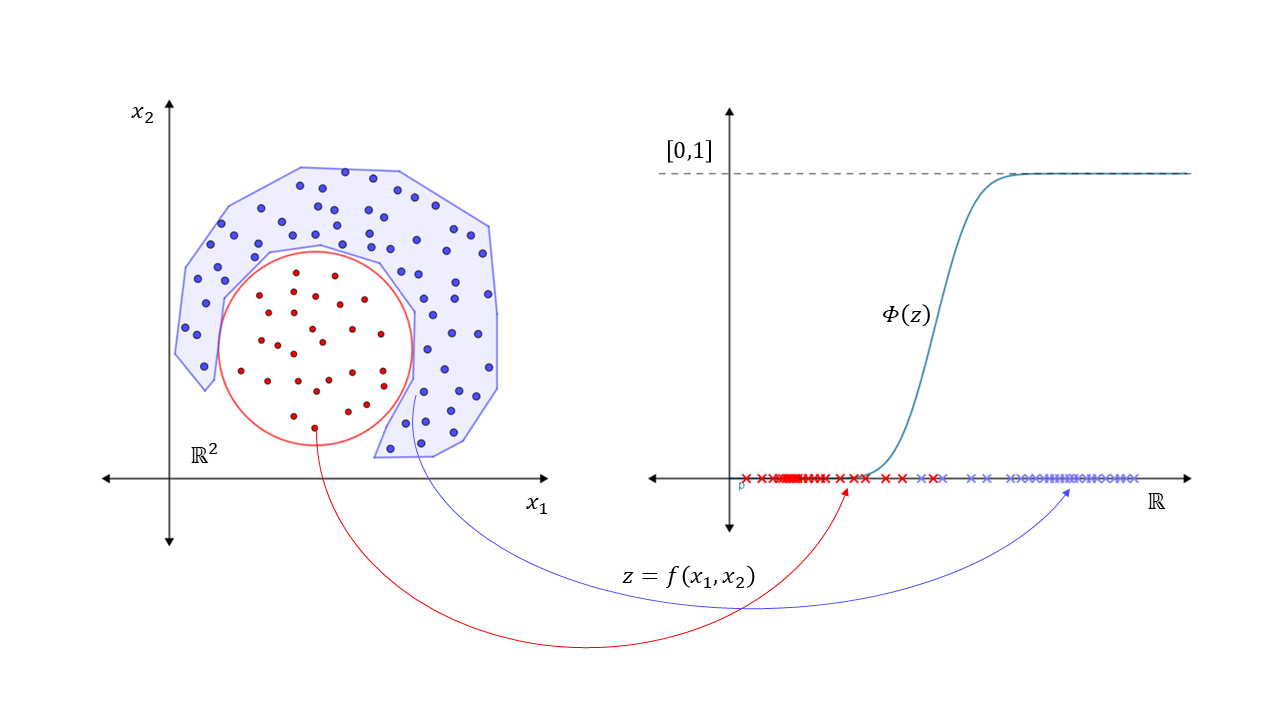
\includegraphics[width = 1\textwidth]{Diagrama_Separabilidad}
  \caption{Diagrama explicativo del modelo. Se tienen observaciones del grupo azul y del grupo rojo con una clara separación no lineal en las covariables $x_1$ y $x_2$. El modelo busca \textit{entrenar} una función $f$ que logre separar lo mejor posible este espacio. Posteriormente, esta separación, induce una clasificación (0 y 1 correspondiendo a rojo y azul respectivamente) a través de la función de acumulación normal $\Phi$, de ahí a que el modelo sea \textit{probit}.}
 \label{fig:DiagramaIntro}
\end{figure}

Es fundamental entender a fondo cada pedazo del modelo, por ello, en el Capítulo \ref{cap:Modelo} se hace una exploración de su forma matemática más rigurosa. Dada su estructura, el modelo  se puede estudiar de arriba hacia abajo, es decir, de la parte más general a la parte más profunda. Por lo tanto, primero se estudian los Modelos Lineales Generalizados (GLM), específicamente los modelos probit. Los GLM dan el salto de una regresión donde la respuesta $y_i$ es real, a regresiones donde la respuesta, puede ser discreta o restringida a cierto dominio \autocite{maccullagh1989generalized}. Los GLM, como su nombre lo indica, siguen siendo lineales, pero este proyector lineal, se puede flexibilizar un poco más usando las ideas de los Modelo Aditivo Generalizado (GAM) presentadas en \autocite{hastie1986generalized}. Los GAM, buscan transformar a las covariables $\xsn_i$, previamente a la regresión, usando métodos no paramétricos. Este trabajo, toma esas ideas y las combina con las de \autocite{mallik1998automatic}, en el que se llevan un paso más allá la transformación para hacerla \textit{tan flexible como sea necesaria}; todo bajo un paradigma de aprendizaje bayesiano. Esta transformación, corresponde a una serie de polinomios por partes de continuidad y grado arbitrarios, sujetos a ciertos nodos, lo cual representa la parte más profunda del modelo. La expansión que se presenta, resulta que conectan muchas disciplinas y ramas de las matemáticas que han sido de mucha utilidad no solo en el campo de la estadística. Al final del Capítulo \ref{cap:Modelo}, se verá que con estos principios se abre un mundo de posibilidades en cuanto a modelos y datos sobre los que se pueden aplicar.\\

Posteriormente en el Capitulo \ref{cap:BayesAlgoritmo}, se hace una breve introducción a la estadistica bayesiana, en particular al apredizaje bayesiano en el contexto de regresión lineal. Esto se debe a que la implementación algorítmica del modelo recae en una técnica fundamental de esta diciplina, el \textit{Gibbs Sampler}, usando las ideas de \autocite{albert1993bayesian}. Con esta poderosa herramienta, se presenta los detalles y lógica del algoritmo. Además, se explica a grandes razgos como se hizo el desarrollo y de un paquete computacional de código abierto en el software \verb|R| para el uso del modelo. El desarrollo de un paquete se detalla en el Apéndice \ref{ap:Paquete}, y corresponde a que, no solo se simplifica la implementación, sino que se está fomentando el fácil uso del modelo y su validación a terceras personas que se puedan interesaran en el. Se hace notar, que al paquete se le añadió funcionalidad adicional para la visualización de ciertas partes del modelo bajo algunos supuestos facilitando su interpretación.\footnote{El paquete se puede descargar libremente de: \url{https://github.com/PaoloLuciano/bpwpm}}\\

Una vez que el modelo fue funcional y fácil de implementar, se probó y se validó contra una serie de bases de datos, tanto simulados como reales para probar su efectividad. En el Capítulo \ref{cap:EjYRes}, se puede estudiar el modelo en una forma más pragmática, pues el uso del paquete lo facilita mucho. En particular, las bases de datos simuladas ejemplifican muy bien el modelo y muestran la flexibilidad de los polinomios por partes logrando encontrar fronteras de clasificación complejas y evidentemente no lineales. Uno de los ejemplos replica de forma fiel, la Figura \ref{fig:DiagramaIntro}.\\ 

Finalmente, en el Capítulo \ref{cap:Conclusiones}, se verán las consideraciones finales y limitaciones del modelo. Sin embargo, se abre una discusión a posibles extensiones para mejorarlo. Posteriormente, se da un vistazo a modelos más modernos los cuales han sido capaces de proezas computacionales que se creían imposibles hace algunas décadas. Se verá, sin embargo, que muchos de los modelos más avanzados y usados hoy en día, son generalizaciones de los modelos tradicionales presentados en este trabajo. Si estos modelos, se comienzan a anidar unos dentro de los otros se logra extender el \textit{aprendizaje} más allá de datos binarios y lograr clasificaciones de imágenes, sonidos y datos poco ortodoxos para la estadística. 
\end{document}

